\documentclass[letterpaper, preprint, paper,11pt]{AAS}	% for preprint proceedings
%\usepackage[latin1]{inputenc}
% These were my imports, can I still use them?
%\usepackage{amsfonts}
\usepackage{amssymb}
\usepackage{graphicx}

\usepackage{bm}
\usepackage{amsmath}
\usepackage{subfigure}
%\usepackage[notref,notcite]{showkeys}  % use this to temporarily show labels
\usepackage[colorlinks=true, pdfstartview=FitV, linkcolor=black, citecolor= black, urlcolor= black]{hyperref}
\usepackage{overcite}
\usepackage{footnpag}			      	% make footnote symbols restart on each page


\PaperNumber{18-269}

% Formatting notes:
% Eq.~(1) or Equation~(1) are both acceptable
% Figure 1, not Fig. or (1)
% 


\begin{document}
\author{Connor D. Noyes\thanks{Ph.D. Student, Department of Mechanical and Aerospace Engineering, University of California, Irvine, 92697} \ and Kenneth D. Mease\thanks{Professor Emeritus, Department of Mechanical and Aerospace Engineering, University of California, Irvine, 92697}} %kmease@uci.edu
\title{A Convex Optimization Approach to Mars Entry Trajectory Updating}
\maketitle
	
	\begin{abstract}
	
	

	\end{abstract}
	
	\section{Introduction}
	Entry, descent, and landing (EDL) capsules traversing the Martian atmosphere are subject to significant uncertainty in the vehicle's aerodynamics, environmental conditions, mass properties, and more that contribute to the difficulty of precision landing for the low lift-to-drag (L/D) ratio vehicles such as those in the class of the Mars Science Laboratory (MSL) mission and the similar Mars2020 mission.\textbf{Add citations for these missions} 
	In addition, delivery errors upon entering the atmosphere mean that tracking a fixed reference trajectory may not deliver the vehicle to the desired target even under nominal conditions. The limited control authority offered by low L/D vehicles is also an added challenge.

	Evidently a closed-looped guidance algorithm is required to tackle these issues. The two major lines of research in recent literature on Mars entry guidance have been reference trajectory tracking and predictor-corrector methods. 
	Although the full merits of each approach are not the subject of this paper, trajectory tracking provides guidance commands in a computationally efficient way but traditionally requires offline design. In contrast, numerical predictor-corrector methods have greater computational requirements but offer high performance and greater adaptability since no reference trajectory is required. 
	
	Of course, not all schemes fit neatly into one of these categories, and the guidance algorithms proposed in the literature increasingly blur the distinction between them by drawing from both methodologies. 
	For example, MSL, the first Mars mission to utilize closed-loop hypersonic entry guidance, employed a variation of the Apollo guidance approach termed the entry terminal point controller (ETPC)\cite{ETPC}. ETPC is considered an analytical predictor-corrector approach but the feedback gains used are dependent on a predefined reference trajectory. 
	Another example from recent literature proposes tracking a trajectory that is designed on-board using a numerical predictor-corrector method\cite{PredictorCorrectorTracking, PredictorCorrectorTracking2}. The benefit of tracking is that replanning is required less frequently and the total computational expense is lower. 
	One final example comes from Reference~\citenum{GuangfeiReplanning} in which a nonlinear predictive drag tracking scheme is augmented with onboard replanning. The results indicate that a low number of updates to the drag profile and bank reversal times provides significant improvement to horizontal accuracy while maintaining high altitude at parachute deploy. 
	
	% Onboard trajectory updating/replanning increases vehicle autonomy, improves performance.
	Convex optimization approaches to solving nonconvex problems have seen immense interest in recent years, \cite{SeqConProg,SuccConvex1,SuccConvex2}, and have been successfully applied in a number of aerospace problems including interplanetary trajectories\cite{wang2018convex}, powered ascent \cite{PS_ConvexAscent} and descent \cite{ConvexDescent} trajectories, as well as atmospheric entry guidance \cite{WangConvexTraj,sagliano2018optimal}. This growth in interest is due to the favorable theoretical and practical properties of convex optimization, namely, that any solution found is a global optimum, and the existence of efficient, polynomial-time solvers for such problems. 
	
	The dynamics of an atmospheric entry vehicle are inherently nonconvex. Treating the vehicle's bank angle as the control variable results in a nonaffine, nonconvex optimization problem. The dynamics are transformed into a convex form by linearization around a reference trajectory. The problem is then fully converted to convex form by treating the bank angle as a system state and using bank angle rate as the control variable as in Reference~\citenum{WangConvexTraj}. Additionally, the formulation here requires a fixed final time. However, the trajectory duration is not in general known \textit{a priori} and the duration may necessarily change during replanning. To remedy this issue, specific energy is used as the independent variable instead of time. Energy is a function of the vehicle's velocity and altitude and a suitable final energy level can be obtained more easily than the trajectory duration, by, e.g., consideration of parachute deployment conditions or supersonic retropropulsion ignition conditions. 
	
	The convex optimal control problem is transcribed into a finite-dimensional problem using \textit{hp} pseudospectral collocation\cite{HP_PS_ConvexDescent} to obtain more accurate solutions for a given number of points than conventional discretization methods like Euler's method \cite{PS_ConvexDescent}. A Chebyshev pseudospectral method \cite{ChebyPS} is used to determine the collocation nodes in each segment, as well the discrete differential and integral operators needed to transcribe the problem. The resulting second-order cone problem (SOCP) \cite{BoydConvexBook} is solved via an efficient interior-point method, implemented in ECOS.\cite{ecos}
	
%	\textbf{Probably need text here to help transition. Describe the proposed approach.}
	We propose the use of convex optimization for the purpose of updating an existing trajectory and in doing so repair any constraint violations while retaining local optimality. 
	Drawing inspiration from the warm starting technique in optimization, the proposed approach is only intended to make corrections to an existing trajectory as needed. As a result it requires an initial trajectory that ``is near" a trajectory that satisfies the constraints. One benefit of the local nature of the update is that feedback gains do not generally need to be recomputed. However, bank reversals can happen at different energy levels and with different rate to produce a new trajectory. The approach also benefits from the fact that all state variables are updated rather than separately addressing the longitudinal and lateral channels as is commonly done. Additionally, only a single convex optimization problem needs to be solved, rather than a series of successive linearizations around the previous solution unlike Refs.~\cite{SeqConProg,SuccConvex1,SuccConvex2,WangConvexTraj}. However, the rapid convergence of these successive approaches from an arbitrary trajectory to an optimal one instills further confidence that a feasible, near-optimal trajectory can be generated from a nearly feasible, nearly optimal trajectory in a single iteration. This makes the algorithm more amenable to real-time implementation. 
	
	The technique proposed here are independent of any particular guidance algorithm, and is expected to be widely applicable. The updating strategy is demonstrated in two different approaches to Mars entry guidance. 
	
% \textbf{A trust region approach is utilized which means the updated trajectory cannot deviate largely from the original. NOT TRUE}

%	The algorithm can also be used for repeated planning and can be seen in the same spirit as the numerical predictor-corrector methods. In this case feedback is achieved by repeated planning from the current vehicle state rather than using numerical prediction to trigger an update to the trajectory. However, in contrast to the standard predictor corrector methods, the profile has the advantage of being more general since the bank angle profile is not constrained by a simple parametrization. This allows for near optimal performance. Nevertheless, the reliance on an initial reference trajectory does ultimately make it less flexible than other predictor-corrector methods. 

%	The cost function in the optimization problem is the sum of a quadratic function of the miss distance from the target and a small control deviation penalty in the Lagrange cost to reduce chattering: 
%	\begin{equation}
%	J = \frac{1}{2}(\theta(E_f)-\theta_{T})^2 + \frac{1}{2}(\phi(E_f)-\phi_{T})^2 + w\int_{E_0}^{E_f}(\Delta u)^2dE
%	\end{equation}
%	where $\theta,\,\phi$ are the vehicle's longitude and latitude, respectively, \textit{w} is an appropriate weighting term, and $\Delta u$ is the update to the control resulting from the optimization procedure. To ensure the final altitude of the vehicle remains sufficiently high during replanning,  it may be treated as a constraint ($h(E_f)>=h_{min}$), or an altitude maximization term may be appended to the cost function. The approach requires a single numerical integration at each guidance cycle to predict the final state under the current plan. This trajectory is then used as the linearization point to convexify the dynamics. Once the replanning is complete, the new trajectory may be tracked via feedback control, or flown open-loop until the next replanning. 
	
	\section{Problem Statement}
	The equations of motion of an entry vehicle defined with respect to a Mars-fixed coordinate frame are 
	\begin{align}
	\dot{r} &= V\sin\gamma\\
	\dot{\theta} &= \frac{V}{r}\frac{\cos\gamma\cos\psi}{\cos\phi}\\
	\dot{\phi} &= \frac{V}{r}\cos\gamma\sin\psi \\
	\dot{V} &= -D - \frac{\mu}{r^2}\sin\gamma \\
	\dot{\gamma} &= \frac{L}{V}\cos\sigma + \left(\frac{V}{r}-\frac{1}{r^2}\right)\cos\gamma \\
	\dot{\psi} &= -\frac{L}{V}\frac{\sin\sigma}{\cos\gamma} - \frac{V}{r}\cos^2\gamma\cos\psi\tan\phi %\\
%	D &= \frac{1}{2}\rho V^2\frac{S}{m}C_d 
	\end{align}
	where $r$ is the radius of the vehicle from the center of Mars, $\theta$ and $\phi$ are longitude and latitude, $V$ is the planet-relative velocity, $\mu$ is the gravitational constant for Mars, $\gamma$ is the relative flight path angle, $\psi$ is the vehicle's heading angle measured counterclockwise from East, and $\sigma$ is the bank angle of the vehicle, defined as the rotation about the vehicle's velocity vector. 
	
%	For lifting vehicles (i.e. nonzero angle of attack), this is different than the roll angle.
	
%	and the differentiation is with respect to nondimensional time. 
%	
%	Proper scaling of the entry states is essential for accurate solutions;
	
	% Trajectory Generation problem
	We seek a bank angle profile that will deliver the vehicle to the target under desirable conditions while extremizing an objective function. For this paper we will consider altitude maximization but note that other convex objectives are possible.
	\begin{align}
		&\max_{\sigma(t)} h(t_f) \label{eq_objective}\\
		&\mathrm{subject\,to\,} \nonumber\\ 
		&\dot{x} = f(x, \sigma) \\
		&|\sigma| \le \sigma_{\max} \\
		&x(t_0) = x_0 \label{eq_initial_cond}\\
		&x(t_f) = g(x(t_f)) \label{eq_terminal_cond}
	\end{align} 
	where $g:\mathbb{R}^n\mapsto\mathbb{R}^p$ defines a terminal manifold specifying any final conditions on the trajectory. $g$ is assumed to be representable into a combination of linear equality constraints and second-order cone constraints. For instance, the conditions on dynamic pressure and Mach number required for safe parachute deployment can be translated into convex bounds on altitude and velocity. 
	
	% Provide motivation for the approach, i.e. that warm starting the optimization will make it converge in a single step
	
	\section{Second-Order Cone Programming}
	% Define SOCP - cite Boyd book?
	% Quadratic forms are converted to cones via norms - cite Stephen Boyd paper 
	A second-order cone program is a convex optimization problem that has the form\cite{BoydConvexBook} 
	\begin{align}
	&\min_z c_0^Tz \label{eq_socp_obj}\\
	&\mathrm{subject\,to\,}\nonumber\\ 
	&||A_iz+b_i||_2\le c_i^Tz + d_i,\quad i=1,...,m \label{eq_cone_constraint}\\
	&Fz=g \label{eq_lin_eq_constraint}
	\end{align}
	where $z\in\mathbb{R}^n$, $A_i\in\mathbb{R}^{n_i\times n}$, and $F\in\mathbb{R}^{p\times n}$. Equation~(\ref{eq_cone_constraint}) defines $m$ $n_i$-dimensional cones, the intersection of which defines a convex feasible space over which the remaining linear program is solved. 
	
	\subsection{Problem Reformulation}
	% Bank angle rate as the control - state now in R7
	The problem as posed is clearly not convex and thus not immediately suitable for solution by convex optimization. The first issue is the control variable $\sigma$ which enters the equations of motion trigonometrically. Following the approach in Reference~\citenum{WangConvexTraj}, the bank rate $\dot{\sigma}$ is taken to be the control and $\sigma$ is treated as an additional system state. The result is a system that is affine in the new control variable and thus more amenable to convex optimization. Since the state dimension is larger, the optimization problem solved at each trajectory update is larger, but the ability to constrain the bank rate and also its acceleration are valuable in generating trajectories that are not only feasible but trackable by the attitude control system. 
	
	% energy as independent variable for fixed final, preferable to velocity since always monotonic 
	As discussed in the introduction, determining a suitable final energy level has advantages over trying to determine an appropriate trajectory duration, motivating our use of energy as the independent variable. Velocity is another candidate, but energy has two advantages. First, velocity is not strictly monotonic from many entry conditions, though in practice any trajectory update would occur deeper in the atmosphere past the point of increasing velocity. Second, delivering the vehicle to a target at a fixed energy rather than a fixed velocity allows for trading off between altitude and velocity. In addition to changing the independent variable, we also nondimensionalize the state vector for better numerical conditioning. The vehicle radius is normalized by the equatorial radius of the planet $R_p$, velocity is normalized by $\sqrt{g_0R_p}$, and time is normalized by $\sqrt{\frac{R_p}{g_0}}$ where $g_0$ is the local gravity acceleration magnitude at $R_p$.
	
	With the inclusion of bank angle as a system state and using nondimensional energy as the independent variable, the equations of motion are
	\begin{align}
	r' &= -\frac{\sin\gamma}{D}\\
	\theta' &= -\frac{1}{rD}\frac{\cos\gamma\cos\psi}{\cos\phi}\\
	\phi' &= -\frac{1}{rD}\cos\gamma\sin\psi \\
	V' &= \frac{1}{V} + \frac{\sin\gamma}{r^2VD} \\
	\gamma' &= -\frac{L}{V^2D}\cos\sigma - \left(\frac{1}{rD}-\frac{1}{r^2VD}\right)\cos\gamma \\
	\psi' &= \frac{L}{V^2D}\frac{\sin\sigma}{\cos\gamma} + \frac{1}{rVD}\cos^2\gamma\cos\psi\tan\phi \\
	\sigma' &= -\frac{u}{VD}
	\end{align}	
	
	% linearization 
	The final step in convexifying the dynamics is to use the Jacobian linearization to produce a linear, energy-varying system:
 	\begin{align}
 	\delta x &= x - x_r \\
 	\delta u &= u - u_r \\
 	A &= \frac{\partial f}{\partial x}|_{\substack{x=x_r\\u=u_r}} \\
	B &= \frac{\partial f}{\partial u}|_{\substack{x=x_r\\u=u_r}} \\
	\delta\dot{x}(E) &= A(E)\delta x(E) + B(E)\delta u(E) \label{eq_LTV_approx}
 	\end{align}
	% Cost function, what to include as a constraint vs terms in objective
%	We choose to enforce the final target latitude and longitude as constraints rather than as penalties in the objective. 
	
	% Discretization via chebyshev polynomial
	In order to convert the convex optimal control problem into a SOCP, the dynamics and Lagrange cost (and path constraints) must be discretized. For this we utilize a Chebyshev pseudospectral method \cite{ChebyPS}. Rather than representing each state with a single global polynomial, a mesh of low-order Chebyshev polynomials is used, i.e., an \textit{hp} pseudospectral method.\cite{HP_PS_ConvexDescent} Since the trajectory update performs only a single iteration, a fixed number and order of polynomials is used, in contrast to \textit{hp}-adaptive methods\cite{darby2011hp}.
	Using a Chebyshev pseudospectral differentiation matrix $D$, the discrete, linearized dynamics are written in the form 
	\begin{align}
	D\delta x = A\delta x + B\delta u
	\end{align}
	which may be rewritten in the form of Eq.~(\ref{eq_lin_eq_constraint}) as follows
	\begin{align}
	z_i& = \left[\begin{array}{c}
	\delta x_i \\
	\delta u_i 
	\end{array}\right] \\
	F_i &= [D-A_i,\,-B_i] \\
	g_i &= 0 \\
	z &= \left[\begin{array}{c}
		 z_0 \\
		\vdots \\
		z_N 
		\end{array}\right]\label{eq_z} \\
	F &= \left[\begin{array}{cccc}
	F_0 &0 &\dots& 0 \\
	0& F_1 &\dots& 0 \\
	\vdots & \vdots &\ddots&0 \\
	0& 0& \dots& F_N \\
	\end{array}\right]	\label{eq_F} \\
	g &= \left[\begin{array}{c}
		g_0 \\
		\vdots \\
		g_N 
		\end{array}\right] \label{eq_g}
	\end{align}

	Additionally, any Lagrange term in the cost function is discretized using Clenshaw-Curtis quadrature
	\begin{equation}
	\int_{E_0}^{E_f} L(x,u)\ \mathrm{d}E \approx \sum_{i=1}^{N}w_iL(x_i,u_i)
	\end{equation}
	where $L:\mathbb{R}^n\times\mathbb{R}^m\mapsto\mathbb{R}$ is a convex function and $w_i$ are the quadrature weights. 
	
	In an \textit{hp} pseudospectral method, the Lagrange term is approximated on each segment. The total integral is then a weighted sum of the segment components, where the weights account for transformation from the independent variable (energy, here) to the ``pseudospectral" time $\tau\in[-1,1]$.
	
	The maximum altitude objective Eq.~(\ref{eq_objective}) can easily be posed in the required form Eq.~(\ref{eq_socp_obj}), and the final target latitude and longitude are expressed as hard equality constraints rather than added as penalty terms in the objective. 
	
	The resulting SOCP consists of the linear objective, the linear dynamic constraints given by Equations~(\ref{eq_z})-(\ref{eq_g}), linear equality constraints on the initial condition (Eq.~(\ref{eq_initial_cond})), and any additional linear or conic constraints due to terminal conditions (Eq.~(\ref{eq_terminal_cond})), path constraints, or trust regions.
	
	Notice that there are no constraints linking the solution at the end of one segment and the solution at the beginning of the next segment. Instead, the same variable is used to represent both values which reduces the total number of constraints.% (the number of segments minus one, times the state dimension). 
	
	\subsection{Implementation Details}
	 The resulting SOCPs are solved via ECOS \cite{ecos}, an interior point solver. We remark that the scaling used to nondimensionalize the state variables is essential to accurate solutions. 
	% Scaling 
	% Trust region size - unlike Ping Lu papers with large trust region 
	
	In practice a small amount of regularization on the control produces higher quality solutions. A Lagrange term is appended to the existing objective functional  
	\begin{align}
	J_{reg} = \alpha\int_{E_0}^{E_f} | \dot{u} | \mathrm{d}E\approx \alpha\sum_{i=1} \left|\frac{u(E_i) - u(E_{i-1})}{E_i - E_{i-1}}\right|  \label{eq_regularize} 
	\end{align}
	where $\alpha$ is an appropriate weighting factor. The solution is not particularly sensitive to this value, typically we take $\alpha\in[1\mathrm{e}-5,\,1\mathrm{e}-2]$. The appropriate range is dependent on the magnitude of the other term(s) of the objective function. After experimentation, we found that the absolute value in Eq.~(\ref{eq_regularize}) is preferable to a quadratic form. In theory, a quadratic penalty should provide similar regularization for an appropriate $\alpha$ but in practice choosing $\alpha$ correctly is difficult and choosing inappropriate values lead to infeasible problems. Similar $ L_1 $-minimization appears in sparse polynomial chaos optimization\cite{SparsePCE}, support vector regularization,\cite{SVM} and compressed sensing.\cite{CompressedSensing} Here it promotes bank angle rate changes as infrequently as possible. Although Eq.~(\ref{eq_regularize}) is not directly in the form required, the absolute value can be reformulated to fit the SOCP structure, see Appendix A for details.  % This could be because of the difference in reformulating these terms? Quadratics become cone constraints while abs become multiple linear constraints 
	
	% \textbf{Since the RCS actuation is discrete this is actually good.}
	
	% Show a figure here, with and without regularization to highlight the impact. Also note that different values of the regularization parameter can be used (good that its robust)
	
	
				\begin{figure}
					\centering
					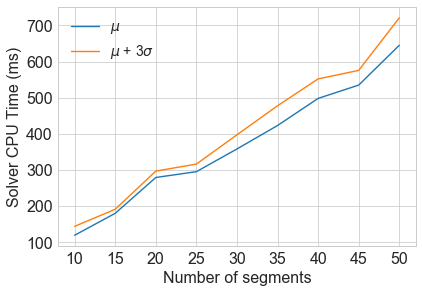
\includegraphics[width=0.75\textwidth,keepaspectratio=true]{solver_times}
					\caption{Solution times for different number of segments using $ \mathbf{4^{th}} $ order Chebyshev polynomials. The average and standard deviation are computed over 20 solutions.}				
					\label{plot_solution_times}
				\end{figure}
	% Size of the mesh used, problem solving time vs size 
	The solution times in Figure~\ref{plot_solution_times} are noticeably longer than those reported in Reference~\citenum{HP_PS_ConvexDescent}, even for the same number of nodes. We should be careful when comparing results as there are several key differences. One is that the entry problems studied here are up to three times longer (in time) than the powered descent problems examined in the reference which necessitates a larger number of nodes for solutions of the same accuracy. Typically a solution cannot be find when the number of nodes is too small, providing too little flexibility to the control. Additionally, the entry dynamics are significantly more nonlinear and coupled due to the presence of trigonometric terms, the atmospheric density model, and aerodynamic forces. Further, the total size of the optimization problems will be different due to the different number of states, controls, and constraints; in particular the entry problem as considered has 7 states and only 1 control while the powered descent problem features 7 states and 4 controls. Finally, different hardware will play a large role in the differences. All problems are solved on an Intel Core i5-7500 CPU at 3.5 GHz.
	
%	Past a certain number of segments, the discretization error becomes negligible compared to the linearization error and the position and velocity errors do not drop any further.
	
	% Additionally, the powered descent problem is fully convexified without the use of linearization in the dynamics 
	
	\subsection{Update Effectiveness vs Energy} \label{Section Reachable Set Analysis}
	Naturally, the benefits of updating the trajectory decrease with energy as the size of the reachable set shrinks. At some point, the remaining energy becomes insufficient to allow significant change. In this section we examine how the efficacy changes along a trajectory. Another key component is determining how much of the reachable set is recoverable by our approach; the difference is due to the linearization step. There exist trajectories that deviate too far from the nominal trajectory to be accurately represented by the linear approximation.  
	
	After each optimization problem, the bank angle solution is integrated numerically to verify satisfaction of the dynamic constraints. Due to the linearization step in formulating the convex problem, some mismatch to be expected. 
	
			\begin{figure}
				\centering
				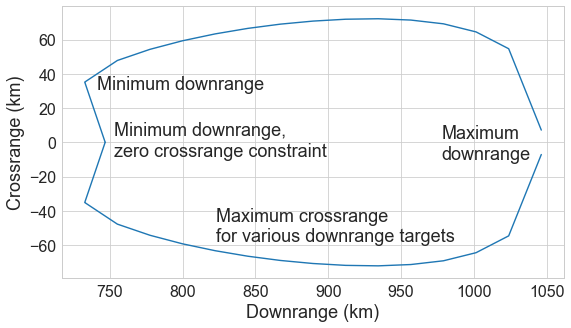
\includegraphics[width=0.95\textwidth,keepaspectratio=true]{reachable_set}
				\caption{An example of a reachable footprint computation.}				
				\label{plot_RS_example}
			\end{figure}
	
	The reachable footprint is a projection of the reachable set onto the longitude and latitude, or equivalently downrange and crossrange. A crude estimate of the reachable footprint for a given initial vehicle state is generated by solving minimum and maximum downrange problems, as well as crossrange maximization problems for a set of downrange values. The final altitude is constrained to be $\ge 7 $km, and the final velocity must be $\le 475$ m/s. Figure~\ref{plot_RS_example} shows an example from an initial velocity of 5400 m/s at an altitude of 55 km. This footprint is used as an estimate of the vehicle's ability to replan its trajectory. The replanning capability in the downrange direction is defined as $\frac{1}{2}(DR_{\max}-DR_{\min})$ and the crossrange capability is simply $ CR_{\max} $. The results are plotted against velocity in Figure~\ref{plot_reachable_radii} for six different entry states. As expected, the downrange capability is larger because the majority of the vehicle's velocity is in the downrange direction at any point along the trajectory. This also explains why it decreases more quickly than the crossrange component as the vehicle decelerates.
	
	From the same initial conditions, various points within the reachable set are chosen as final conditions in the convex optimization problem. 
	
		\begin{figure}
		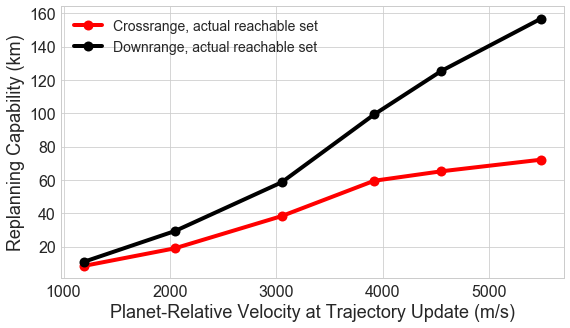
\includegraphics[width=0.95\textwidth,keepaspectratio=true]{reachable_radii}
		\caption{The true reachable downrange and crossrange capabilities of the vehicle decrease as a function of velocity. The capability is half of the true reachable footprint's size in each direction.}
		\label{plot_reachable_radii}
		\end{figure}
	
	As velocity decreases, the convex trajectory update can reach a larger fraction of the reachable set. This is primarily due to two reasons. The remaining length of the trajectory is shortened, so errors due to linearization have less time to accumulate. The reachable set itself is smaller, and thus the linearization is valid over a larger portion of the set. 



	
	% Two approachs - set a threshold, and anything under it is sufficiently accurate
	% Or, simply define a metric (integral of difference between cvx vs integrated) and show how the metric changes 
	
	
	% These results could be used to determine how much deviation is acceptable before we must replan 
	
	%	True footprint via gpops vs "single" replanning  as a function of the remaining energy?
	
	% Plot the diameter of CR and DR of reachable set vs enery level (or velocity as a more readable proxy)
	
	% Can also consider something like the ratio of horizontal correction (how much DR/CR need to change during replanning) vs the accumulated error during the replan? 
	
	% How to deal with different parameters? Take jacobian with respect to params and incorporate somehow?
	
	\section{Numerical Demonstrations}
	\subsection{Models}
	The problems are demonstrated using a vehicle in the class of MSL and M2020. The Martian atmosphere is modeled using MarsGRAM.\cite{MarsGRAM2010,MarsGRAM2010User} Lift and drag coefficients are modeled assuming a fixed angle of attack profile and are computed as a function of Mach number from MSL curve fit data. The bank angle rate is limited to $20^{\circ}/s$. The final energy targeted is a result of parachute conditions; we use the same conditions that MSL was subject to, i.e., dynamic pressure between 300 and 800 Pa and Mach number between 1.4 and 2.2. 
	
	The initial reference trajectory is designed using the algorithm in this paper but with iteration until convergence using the virtual control safeguarding technique described in Reference~\citenum{SuccConvex1}. This safeguard is essential for preventing infeasibility in early iterations where the trajectory used for linearization is far from satisfying the constraints. The weight in the exact penalty is a constant 1e4.
	% Similarly, any trust region constraints must contain a feasible point.  Sounds stupid/obvious when worded this way. For example, TR on lat/lon must contain the target lat/lon from the linearized value. 
	
	\subsection{Example 1: Delivery Error Correction}
%	 Simple case study -  delivery error in entry FPA (and maybe others), fly till 0.2g drag level and trigger a replanning to compensate the predicted errors. Do a small monte carlo open loop then show the corrections via convex. Can also give the computation time average and std. 
	%	Be sneaky by using the largest error correction possible based on the results on the previous section.

	% Plot the original trajectory, the predicted trajectory at 0.2g, and then the updated trajectory 	
	For simple exposition, a Monte Carlo is conducted for various entry states. The trajectory is propagated open-loop until 2 $ \mathrm{m/s}^2 $ of drag acceleration is sensed. The errors accumulated from the entry state dispersions are compensated by the trajectory update. 

	
%	The replanned solution often displays a control that differs largely at the beginning and converges toward the original at the end. This is due to the fact that the Lagrange term is integrated with respect to energy. 
	\subsection{Example 2: Drag Tracking with Convex Trajectory Updating}
	Drag tracking provides a robust way to control the vehicle's range but does not consider altitude performance nor does it provide lateral control. The addition of trajectory updating can remedy both of these deficiencies. The use of optimization ensures excellent altitude performance while driving horizontal error to zero. 
	
	The nonlinear predictive control described in Reference~\citenum{benito2008nonlinear} is implemented without the range-to-go component, analogous to omitting the integral term of a PID controller. When used for reference updating in a tracking scheme, some margin should be preserved for tracking, naturally. We thus choose $\sigma_{\max}=81^{\circ}$. Bank reversals are commanded at the same energy level as the latest trajectory update. 
	
	Periodically, the equations of motion are integrated until the final energy level is reached using the reference bank profile. When the predicted miss distance is larger than a threshold value, a trajectory update is triggered. In general, the numerical prediction need not be performed at the same rate as the feedback commands, e.g., if the GNC system generates new bank angle commands at 1 Hz, the update trigger could be checked at 0.2 Hz. In addition to its use in triggering an update, the result of the forward integration is used as the linearization point. In order to better handle parametric uncertainties, the forward integration is carried out using a fading memory filter for the lift and drag accelerations based on the discrepancy between the value measured onboard and the modeled value.\cite{lu2014entry}
	
%	How to trigger the update? One possibility is use to the difference between the estimated range to go and the reference value at the same energy level. A different approach would be to numerically integrate the reference bank profile forward (including the effects of lift/drag filters) to predict error in both downrange and crossrange. This is mildly more computational but has numerous advantages. Additionally, even with the first method, an integration should be performed for the linearization step.  
		 
		 	% Then consider parametric uncertainty and show that multiple replannings helps 
	\subsection{Example 3: Locally Optimal Predictor-Corrector}
	Rather than use an explicit feedback controller as in the last section, a different approach is to use trajectory updating at a fixed rate. Since there is no trajectory tracking, the bank angle profile need not reserve margin so we set $\sigma_{\max}=90^{\circ}$.
	In a PC approach, if the planning is too infrequent then a single iteration may not suffice. A sufficient rate can be determined based on the analysis in Section~\ref{Section Reachable Set Analysis}.
	 
	 The tradeoff is increased computational expense. Even at a low guidance cycle of 1 Hz, the current approach may not be viable for current generation hardware. 
	
	
%	\subsection{Discussion} % Maybe this should just be the conclusion? 
	\section{Conclusion}
	
	\section{Acknowledgments}
	Financial support from the Holmes Endowed Fellowship is gratefully acknowledged.

	\appendix
	\section{Appendix A: Reformulating Sums of Absolute Values}

	Minimization of a sum of absolute values such as 
	\begin{align}
	\min_x\quad &\sum^N_{i=1}|x_i| \\
		&\mathrm{subject\,to\,} \nonumber\\
		&Kx \le c 
	\end{align}
	can be posed in the desired conic form by introducing $N$ auxiliary variables $s_i$, and defining $2N$ additional constraints resulting in the following SOCP\cite{BoydConvexBook}
	\begin{align}
	\min_x\quad &\sum^N_{i=1}s_i \\
	&\mathrm{subject}\,\mathrm{to}\, \nonumber\\
	&Kx \le c \\
	&s_i \ge x_i , \quad i=1,\dots,N\\
	-&s_i \le x_i, \quad i=1,\dots,N 
	\end{align}
		
	Similarly, constraints on sums of absolute values, i.e., $\sum^N_{i=1}|x_i|\le b$, can also be replaced by using $N$ new variables $ t_i $, and $2N+1$ additional constraints 
	\begin{align}
	&\sum^N_{i=1} t_i \le b \\
	&t_i \ge x_i, \quad i=1,\dots,N\\
	-&t_i \le x_i ,\quad i=1,\dots,N
	\end{align}
	
	\section{Appendix B: Reformulating Quadratic Forms}
	Minimization of a quadratic form such as 
	\begin{align}
	\min_x\quad &x^TAx + b^Tx \\
		&\mathrm{subject\,to\,} \nonumber\\
		&Kx \le c 
	\end{align}
	where $A$ is a positive semidefinite matrix can be reformulated as an SOCP as\cite{BoydConvexBook}
	\begin{align}
	\min_{x,y,u}\quad &y + b^Tx \\
	&\mathrm{subject\,to\,} \nonumber\\
	&Kx \le c \\
	&\left|\left|\begin{array}{c}
	2u \\y-1
	\end{array}\right|\right|_2 \le y + 1 \\ % This weird thing is a reformulation of the more simple u^tu \le y
	&u=L^Tx
	\end{align}
	where $LL^T=A$ is the Cholesky factorization of A.
	
		
		\bibliography{bib}
		\bibliographystyle{AAS_publication}
	
		
%		S. Boyd, C. Crusius, and A. Hansson, ``Control Applications of Nonlinear Convex Programming"
		
%		\bibitem{CCQuad}
%		W.M. Gentleman, ``Algorithm 424: Clenshaw-Curtis quadrature [D1]"

\end{document}